%%%%%%%%%%%%%%%%%%%%%%%%%%%%%%%%%%%%%%%%%%%%%%%%%%%
%% Présentation du projet
%%%%%%%%%%%%%%%%%%%%%%%%%%%%%%%%%%%%%%%%%%%%%%%%%%%
%%%%%%%%%%%%%%%%%%
\section{Présentation du projet}
\addcontentsline{toc}{subsection}{Introduction}
\subsection*{Introduction}
Dans ce présent chapitre, nous nous articulerons sur l’étude et l’analyse du projet.
Pour ce faire, nous débuterons par une étude préalable dans laquelle nous exposerons les fonctionnalités de la GED et ses avantages compte tenu de son implication dans le sujet, puis nous entamerons une étude du système existant, pour ensuite identifier les problèmes, les points à améliorer et les solutions envisagées.
\subsection{Étude préliminaire}
Avant d'entamer la discussion sur le sujet du stage, nous allons introduire quelques concepts et terminologie de la GED qui nous aideront à mieux comprendre le sujet par la suite.
\subsubsection{Qu'est-ce que la GED ?}
\begin{beware}[title=Définition : ]
    La GED ou Gestion Électronique de Documents est ensemble de logiciels concourant à réaliser les diverses étapes de la chaîne de traitement d’un document : acquisition, restitution, diffusion \cite{ged}.
    \end{beware}
    La GED est donc un système informatique qui vise à
    gérer et organiser les documents numériques (souvent issus de l'entreprise). En outre, la GED permet la numérisation des documents papier, ainsi que la dématérialisation des processus métier associés.\\La gestion électronique des documents utilise des outils et des fonctionnalités pour gérer toutes les étapes du cycle de vie d'un document numérique :
\begin{itemize}
    \item Création ou acquisition du document (ex : numérisation) ;
    \item Stockage, indexation et organisation du document électronique ;
    \item Gestion de la sécurité des données du document électronique ;
    \item Recherche, consultation du document électronique et échange des informations ;
    \item Archivage électronique du document durant son délai de conservation.
\end{itemize}
\subsubsection{Bénéfices d'une GED}
D’un point de vue stratégique, la mise en place d’une solution de GED rend possible une rationalisation des flux d’informations et donc un gain de temps. Elle permet notamment de :    
\begin{itemize}
    \item Éviter la duplication des processus et ainsi réduire les coûts de traitement.
    \item Éviter la perte de documents.
    \item Trouver facilement et rapidement la bonne version d’un document.
    \item Uniformiser les pratiques documentaires.
    \item Partager des données avec un certain nombre de personnes autorisées.\\
\end{itemize}

D’un point de vue plus opérationnel et technique, la GED garantit : 
\begin{itemize}
    \item La pérennité des documents et de leur support.
    \item L'interopérabilité : les documents peuvent être accessibles sur différentes plates-formes et pour des usages divers.
    \item La sécurité : l’accès aux données est sécurisé, la solution s’adapte aux différents profils utilisateurs.
    \item La traçabilité : retrouver les actions effectuées (dépôts, restitutions, demandes de copies, etc.)
\end{itemize}
\subsection{Étude de l'existant}
\subsubsection{Présentation du projet Arkevia}
\textbf{ARKEVIA} est  un service  innovant  et  pratique de coffre-fort  numérique  développé  par  Cegedim  SRH permettant aux salariés des entreprises adhérentes de recevoir et de conserver dans un espace sécurisé les bulletins de salaire et les communications institutionnelles en version électronique dans des conditions optimales de confidentialité et de sécurité. Arkevia permet également aux salariés de classer et de conserver leurs documents personnels importants tels que les pièces d'identité, les diplômes, les factures, etc.\\

Le coffre-fort Arkevia constitue un espace de stockage sécurisé pour les documents qui y sont déposés (EDI, EDI signé, PDF signé).\\
Il permet de garantir :
\begin{itemize}
    \item \textbf{Intégrité} : L'intégrité des documents, au moyen d’une fonction de signature électronique.
    \item \textbf{Confidentialité} : La confidentialité des documents, au moyen d’une fonction de chiffrement de données.
    \item \textbf{Traçabilité} : La traçabilité des actions effectuées (dépôts, restitutions, demandes de copies, etc.)
    \item \textbf{Vocation probante} : Les solutions de traçabilité constituent de vraies preuves juridiques basées sur leur intégrité, leur exhaustivité et leur opposabilité en cas de litige.\\
\end{itemize}
\newpage
\noindent
\textbf{Bénéfices pour le salarié :}
\begin{itemize}
    \item Accès illimité (24 h/7 j) depuis n’importe quel endroit grâce à une connexion Internet.
    \item Tous les bulletins de salaire déposés dans le coffre-fort ont la même valeur juridique que leur équivalent papier, même en cas de départ de l’entreprise.
    \item Espace personnel sécurisé de 1 Go dédié pour archiver les bulletins de paie et documents RH en version électronique pour une durée de conservation peut aller jusqu'à 50 ans des bulletins de salaire.
    \item Protection des documents importants contre le vol et la perte.
    \item Accès au coffre-fort sécurisé et garanti.\\
\end{itemize}

\noindent
\textbf{Bénéfices pour l’entreprise :}
\begin{itemize}
    \item Optimisation des processus RH d’éditique et de distribution documentaire.
    \item Réduction des coûts de distribution.
    \item Image moderne et innovante de la DRH.
    \item Enrichissement de l’expérience du salarié.
\end{itemize}
\subsubsection{Architecture globale d'Arkevia}
Terminologie nécessaire à la compréhension du sujet :
\begin{beware}[title=Terminologie : ] 
   \begin{itemize}
       \item \textbf{SignArchive} : application de la BU Cegedim e-business, hostée au  datacenter de Boulogne et exploitée par l’équipe interne, ayant pour but le stockage et la signature de documents numériques dans des services à valeur légalement probante.
       \item \textbf{Arkevia} : application Web, décrite dans ce document, présentant une  interface web publique consultable par un navigateur, dont le but est l'exploration et la manipulation de documents dans les coffres SignArchive.
       \item \textbf{Arkevia-SRH} : module d'extension pour Arkevia permettant la mise à disposition dans Arkevia de données (traductions, formulaires d’abonnement, conditions  d'utilisation) issues du système d’information de SRH. Ce module permet la prise en charge des abonnements des utilisateurs d’Arkevia au système de dématérialisation des bulletins de paie émis par SRH.
       \item \textbf{SignArchive-Batcher} : module de traitement générique pour les   applications souhaitant émettre des documents dans SignArchive, à des fins d’exploration par un utilisateur Arkevia.  Le système d’information de SRH utilise SignArchive-Batcher pour placer les bulletins dans les coffres.
   \end{itemize}
\end{beware}
\subsubsubsection{Généralités}
Le développement du produit SignArchive offre à la BU Cegedim e-business, ses clients et partenaires, l’occasion de disposer d’un produit capable à la fois :
\begin{itemize}
    \item de stocker des fichiers (de façon légalement probante si besoin) ;
    \item de les organiser par des métadonnées ;
    \item de fédérer des droits d’accès dynamiques autour de ces fichiers via une API standard (purement HTTP).
\end{itemize}
Au-delà de l’aspect juridique de ce logiciel d’archivage (exploité par les solutions de dématérialisation du groupe), le groupe dispose également d’un moteur de stockage, gestion, recherche et contrôle d'accès qui peut être mis à disposition de toute problématique orientée partage ou publication de document.\\

C’est à une de ces fonctions que s’attache  le projet  Arkevia,  dont  le périmètre fonctionnel est triple :
\begin{enumerate}
    \item Fournir un site web portant une offre de coffre-fort numérique à destination du (grand) public et exposé via le produit SignArchive. Ce site web s’appelle Arkevia.
    \item Offrir à des tiers la capacité de devenir « producteur de documents » pour le portail Arkevia, c’est-à-dire, définir les modalités techniques selon lesquelles un système d’information (interne ou externe) peut s’accrocher au portail Arkevia et à SignArchive,  de façon à ce que les clients d’Arkevia puissent visualiser des documents produits par des tiers.
    \item Implémenter un  tel « tiers producteur » pour les besoins de SRH, permettant la dématérialisation des bulletins de paie émis par l’entreprise.\\
\end{enumerate}

Le deuxième point définit clairement l'objectif d'extensibilité du système, ce qui détermine la plupart des choix de mise en œuvre effectués pour parvenir à la solution globale.

\subsubsubsection{Présentation métier}
La réalisation de la finalité du produit, à   cause de son besoin de généricité, est confiée à trois livrables distincts.
\begin{beware}[title=Note : ]
    La présence de ces trois produits est nécessaire au fonctionnement global de la solution Arkevia+SRH, mais Arkevia peut/aurait pu/pourrait tout à fait exister sans le module SRH, et réciproquement, le module SRH n’a pas besoin d’Arkevia pour pousser les fichiers dans les coffres SignArchive. D’autre part, le module SRH a été développé par Cegedim e-business à la demande de SRH, mais le produit est conçu de sorte qu’Arkevia puisse être implémenté par un producteur qui souhaite prendre en charge lui-même cette implémentation.
\end{beware}
\noindent
Ainsi, les fonctionnalités sont réparties comme suit :\\\\
\textbf{Arkevia}\\
Le site web Arkevia  propose à des navigateurs web en provenance d’internet, la consultation de coffres-forts  SignArchive dans  une interface  de navigation  proche d’un explorateur. Son rôle premier est  donc celui  de « proxy » SignArchive (se connecter pour le compte de l’utilisateur sur SignArchive), et de couche de présentation. D’autre part, Arkevia permet à ses utilisateurs de « s’abonner » à des « producteurs » de documents. La gestion de ces abonnements (présentation  du formulaire d’abonnement spécifique à un producteur, messages de notification du  producteur, ...) nécessite qu’Arkevia puisse communiquer avec le producteur pour échanger images, documents, données, etc. Cette communication doit respecter des principes techniques établis dans le cahier des charges d'implémentation d’Arkevia.\\\\
\textbf{Arkevia-SRH}\\
Ce livrable constitue le module d’abonnement du producteur SRH. Son rôle est :
\begin{enumerate}
    \item De gérer la liste des personnes autorisées à s’abonner au producteur SRH ; et d'en rendre compte à SRH.
    \item De fournir à Arkevia les éléments nécessaires à la  présentation  et la  prise en compte des données d’abonnement (champs de formulaire à  présenter pour s'inscrire, libellés traduits des messages affichés par \textbf{Arkevia} pour le compte de SRH, etc.).
\end{enumerate}

Il est donc constitué à la fois d’une chaîne de traitement chargée de la prise en compte des données d’inscription publiées par SRH, et de web services de publication de données.\\\\
\textbf{SignArchive-Batcher}\\
Ce livrable est une chaîne de traitement publiant, pour le compte de SRH, les bulletins de salaire à dématérialiser dans \textbf{SignArchive}, selon le format admissible pour \textbf{Arkevia}.\\\\
\subsubsubsection{Vue d’ensemble}
Au global, on a une répartition des tâches sous la forme schématique suivante (voir figure  ~\ref{fig:architecture_arkevia}) :
\begin{figure}[H]
    \begin{center}
        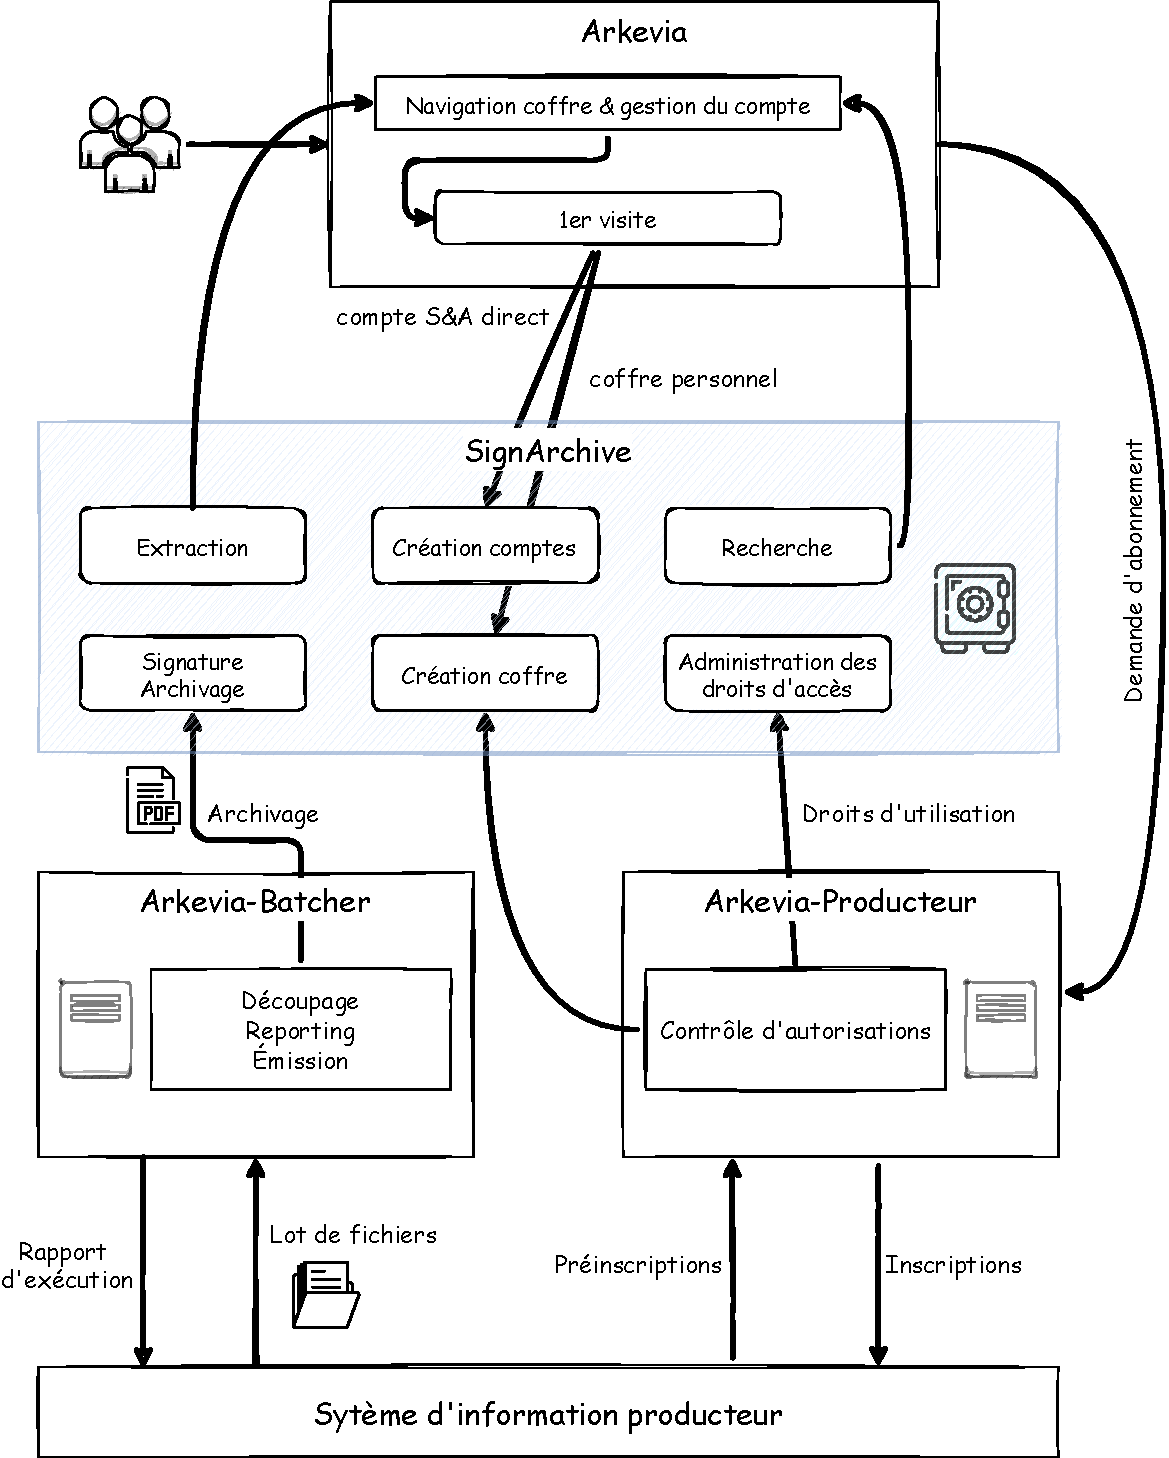
\includegraphics[width=\linewidth]{images/sec2/architecture-globale.pdf}
        \caption{Répartition des tâches dans l'écosystème Arkevia}
        \label{fig:architecture_arkevia}
    \end{center}
\end{figure}
\newpage

\begin{enumerate}
    \item  \textbf{Arkevia} se connecte à \textbf{SignArchive} pour en afficher le contenu, indépendamment du fait que SRH publie ou non des documents pour cet utilisateur. Cependant, si l’utilisateur souhaite s’abonner au service de production SRH, alors, Arkevia pousse la demande via un web service au module approprié, \textbf{Arkevia-SRH}.

    \item \textbf{Arkevia-Producteur (Arkevia-SRH)} peut prendre en compte ou non la demande, selon les autorisations qui lui ont été publiées par SRH directement, via le fichier des préinscriptions. Chaque inscription ou résiliation est remontée à SRH via le même canal que le fichier des préinscriptions.

    \item En conséquence de quoi, lors de la fabrication des bulletins de paie, le module de gestion interne à SRH peut constituer une archive des bulletins à archiver conforme aux utilisateurs Arkevia inscrits. Ce fichier est poussé au module \textbf{SignArchive-Batcher} qui pousse les fichiers dans \textbf{SignArchive}.
\end{enumerate}
\subsubsection{Modules applicatifs}
Arkevia est composée de huit modules permettant de gérer les différents aspects de l'application.
\begin{figure}[H]
    \begin{center}
        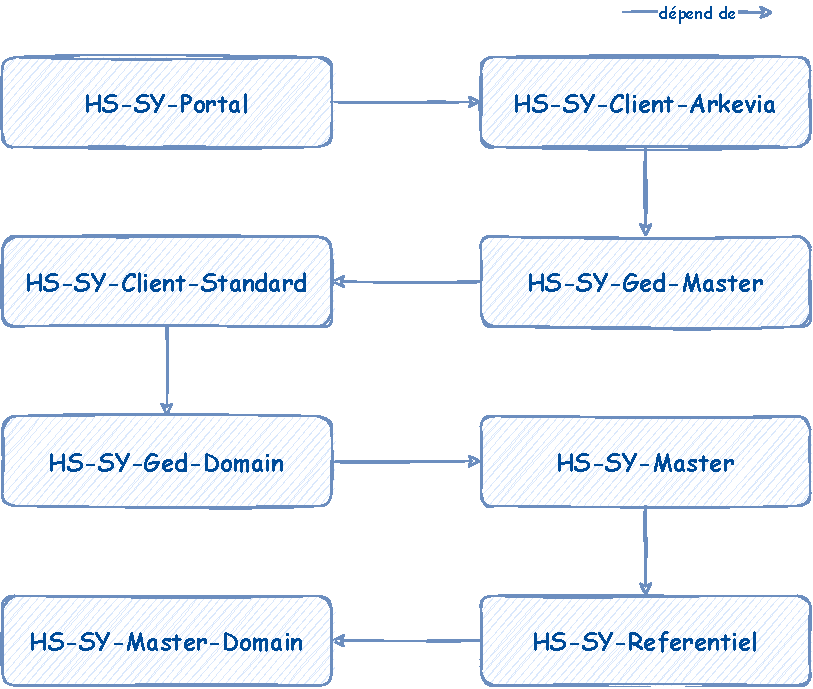
\includegraphics[width=0.56\linewidth]{images/sec2/modules-arkevia.pdf}
        \caption{Architecture modulaire d'Arkevia}
        \label{fig:modules_arkevia}
    \end{center}
\end{figure}
\begin{itemize}
    \item \textbf{HS-SY-Portal}
    Ce module contient tous les éléments qui composent le corps du front-end Arkevia, y compris les composants Vue, les scripts, les images et les feuilles de style.
    \item \textbf{HS-SY-Client-Arkevia}
    Ce module regroupe tous les services propres au client Arkevia, notamment l'inscription, la désactivation du compte, l'exportation de documents, etc.
    \item \textbf{HS-SY-Ged-Master}
    Ce module comprend les services de gestion des répertoires et des documents, y compris la consommation de l'API SignArchive.
    \item \textbf{HS-SY-Client-Standard}
    Ce module comprend tous les services standards et les classes d'écran utilisés dans l'application.
\end{itemize}
Master
Ce module regroupe les services de configuration, d'authentification, de gestion de compte ...

Master-Domain
Ce module gère les interactions avec la base de données, il regroupe toutes les entités qui servent à faire le mapping avec les tables.

On trouve aussi l'ensemble des objets d'accès aux données.

Ged-Domain
Ce module regroupe toutes les entités spécifiques pour la gestion des documents, qui servent à faire le mapping avec les tables.


Referentiel
(Deprecated)






\subsection{Problèmes et axes d'amélioration}
\subsubsection{Défis technologiques}
Le backend de l'application Arkevia est développé principalement avec la technologie Spring 3.x. Ce framework a été publié pour la première fois en 2004 et a subi de nombreuses révisions depuis lors : 
\begin{itemize}
    \item Spring 2.0 a fourni des espaces de noms XML et le support d'AspectJ ; 
    \item Spring 2.5 a adopté la configuration basée sur les annotations ; 
    \item Spring 3.0 a introduit une solide base Java 5+ à travers le socle du framework et des fonctionnalités telles que le modèle @Configuration basé sur Java.\\
\end{itemize}

Aujourd'hui, le projet Spring et le développement Java ont tous deux évolué de manière significative, incluant à la fois des correctifs de sécurité et de nouvelles fonctionnalités et améliorations, faisant de la migration une tâche assez importante.

À cet égard, il a été convenu de réaliser une étude comparative sur l'impact d'une telle migration du framework Spring ; le résultat de cette étude fera l'objet d'un travail de développement sur la migration du socle technique d'Arkevia.

\subsubsection{Refactorisation et nettoyage du code}
Comme mentionné dans l'introduction, le portail Arkevia a subi plusieurs changements et évolutions au cours des dernières années, rendant le code trop compliqué, redondant et imprégné de mauvaises odeurs (code smells), d'où la nécessité de recourir à un processus de refactoring et d'amélioration du code tout en préservant les fonctionnalités existantes. Le but est de transformer un code inefficace et compliqué en un code plus efficace, de préférence plus simple et plus facile.
\subsubsection{Mécanisme de Notification}
Le mécanisme d'envoi de notifications est responsable de notifier un utilisateur par mail, lorsqu'il y a un nouveau dépôt de document (Bulletin de paie, note de frais, etc.) sur son coffre-fort par la société à laquelle il appartient.\\

Le module de gestion de l'envoi des notifications est intégré à l'application mère Arkevia. Le processus d'envoi est planifié pour être déclenché toutes les deux heures, et à chaque exécution, l'application Arkevia sollicite le service chargé d'interroger l'API SignArchive pour récupérer la liste des documents déposés et celle des utilisateurs associés afin de préluder à l'envoi des notifications.
Le mécanisme actuel n'est pas capable à traiter la volumétrie de documents en production. En effet, ce dernier souffre de plusieurs failles et notamment quand le nombre de documents déposés dans SignArchive est élevé, le système se met à défaillir et à dysfonctionner, ce qui entraîne que certains utilisateurs ne reçoivent plus les notifications sur la présence des documents déposés dans leur coffre-fort ou les reçoivent plusieurs fois pour un même document, etc. 

\subsection{Objectif de la refonte}
L'objectif est de revoir, corriger et améliorer / traiter les problèmes et les axes d'amélioration identifiés suite à l'audit d'architecture effectué.

Avec un refactoring continu qui adopte une approche progressive, le produit reste utilisable, contrairement à un logiciel qui doit être entièrement réarchitecturé, voire redéveloppé. Comme je l’ai dit, je pense que c’est la meilleure option pour pérenniser un produit digital mais ce n’est pas une solution miracle. Elle demande du temps et des compétences, quitte à reporter le développement de certaines nouvelles fonctionnalités.

Si je peux donner un conseil sur l’organisation, ce serait de garder un temps au refactoring de code dans chaque itération et quand c’est nécessaire lui réserver une itération.
\addcontentsline{toc}{subsection}{Conclusion}
\subsection*{Conclusion}
%%%%%%%%%%%%%%%%%%%%%%%%%%%%%%%%%%%%%%%%%%%%%%%%%%%

